%Architectural Design section

\subsection{Overview}
% High level components and their interactions

This chapter will illustrate the architecture of the system with its logical and physical components and how they interact to reach the goals. The sections of this chapter are:
\begin{itemize}
	\item High level components and their interactions: it provides a general idea about the physical components of the system
	\item Component view: it shows the strctures of the logical components and how they communicate with each other
	\item Deployment view: it describes the physical structure of the system and shows where each component will be deployed. It will also present the possible technologies that will be used for the implementation.
	\item Runtime view: it presents how the components communicate with each other inside the most important scenarios that will be handled by the application
	\item Component interfaces: it describes the interfaces between the components of the system
	\item Selected architectural styles and patterns: it explains the patterns and architectural paradigms that have been used in some aspects of the architectural desig
	\item Other design decisions: it presents further design choices that are worth mentioning
\end{itemize}

\subsection{High level components and their interactions}

The high level structure of the system follows a three-tier architecture. The client side is developed as a website and a mobile application, which are the interface of the user to the services of the system. The server contains all the business logic and is divided into several components. Each of them has a specific role and acts as an interface for other components and uses the interface provided by other components. Some other services participate in the functioning of the system but are outside the server: these are the external services, used for calculating routes, solve addresses into GPS coordinates and checking the weather conditions. Other external components let the application send push notification and SMS to the phone of a user. Finally, the last tier is realized by the database server, which is external to the main server hosting the business logic.

\subsection{Component view}

\begin{figure}
\centering
\includegraphics[width=\textwidth]{{"Images/Architecture - Component View"}.png}
\caption{\label{fig:metamodel2}Component diagram of the system}
\end{figure}

\begin{itemize}
	\item Web Application: client side component for the application via web browser
	\item Mobile Application: client side component for the application via mobile device
	\item SessionManager: handles login, sign up and general account functionalities
	\item NotificationManager: handles notifications for weather forecast, incoming routes and account recovering by phone number
	\item CalendarManager: handles the calendar and its appointments
	\item RouteManager: handles routes and their generation
	\item ReportManager: handles functionalities for reporting issues and suggestions
	\item PreferenceManager: handles the settings of the user, in particular for route computation
	\item SMS Gateway: service for sending SMS
	\item Push Gateway: service for sending push notifications
	\item Weather Services: external API for weather forecast
	\item Map Services: external API for maps
	\item Route Services: external API for routing
	\item Database: the database of the system
\end{itemize}

The SessionManager exposes an interface for client users and it is a sort of dispatcher of the requests, since the available functionalities are different for registered users and normal users.

All the functionalities of the system are divided among the corresponding manager. The need some external services for fulfilling their task, which are represented as external components. Other external components are the Push Gateway and the SMS Gateway, which are not mandatory but provide a better user experience.

\subsection{Deployment view}

The architecture is divided in the following tiers:
\begin{itemize}
	\item Client tier: it is the interface of the application to the user, executable as a website on a browser or a graphical interface on a mobile device. The website is realized with the classical tools HTML5 and CSS, while the mobile application is available on Android and iOS operating systems.
	\item Web tier: it contains the web server which receives the HTTP requests from the web client and answers with HTML pages generated by a script engine. It can be implemented by the Tomcat web server and the JSP containers of Java EE.
	\item Application tier: it contains the core of the application with all the running components. It can be implemented using the Glassfish application server and the logic is contained in stateless Java beans. The communication with database happens with the JPA interface.
	\item Database tier: it contains the DBMS with the persistent data. It is accessible only by the application tier. A possible implementation will use the MySQL database.
\end{itemize}

\begin{figure}
\centering
\includegraphics[width=\textwidth]{{"Images/Architecture - Deployment View"}.png}
\caption{\label{fig:metamodel2}Deployment diagram of the proposed implementation}
\end{figure}

\subsection{Runtime view}
%Sequence diagrams to describe the way components interact to accomplish each task from use cases

The following sequence diagrams show the interaction between the components of the system while fulfilling the main features of the application. The features have been chosen in such a way that every component appears at least once in any sequence diagram, so that every component can be observed while operating in a scenario.

\begin{figure}
\centering
\includegraphics[width=\textwidth]{{"Images/Architecture - Runtime View - Log in"}.png}
\caption{\label{fig:metamodel2}User login}
\end{figure}

\begin{figure}
\centering
\includegraphics[width=\textwidth]{{"Images/Architecture - Runtime View - Add appointment"}.png}
\caption{\label{fig:metamodel2}Add an appointment}
\end{figure}

\begin{figure}
\centering
\includegraphics[width=\textwidth]{{"Images/Architecture - Runtime View - Add route"}.png}
\caption{\label{fig:metamodel2}Add a route}
\end{figure}

\begin{figure}
\centering
\includegraphics[width=\textwidth]{{"Images/Architecture - Runtime View - Notification"}.png}
\caption{\label{fig:metamodel2}Send a notification (push or SMS)}
\end{figure}

\subsection{Component interfaces}

As shown in the component diagram, all components are interconnected. Here follows an explanation of the services offered and used by each component.

\begin{itemize}
	\item The SessionManager offers an interface to the client tier. It gives the possibility for a user to login or sign up, using also the phone number. All the requests made by a user pass through this interface, checking if a user has the right to make that request and then forwarding it to the correct component.
	\item The NotificationManager offers methods to send push notifications and SMS messages. These methods are used by the SessionManager for allowing a user to login with a phone number, and by the CalendarManager to warn a user that a registered appointment or route is going to begin. This component relies on external services for delivering the messages.
	\item The CalendarManager is the container of the methods to handle the calendar and the appointments. It uses the interfaces of RouteManager and ReportManager for managing routes and reporting issues. Also map services are required when solving the addresses of the appointments.
	\item The RouteManager has the task to create, calculate and manipulate routes according to the needs of a user. It needs the external map and routing services and uses the PreferenceManager to get the necessary constraints while building a route.
	\item The PreferenceManager allows to create and manage the preference profiles of a user.
	\item The ReportManager allows to register issues, reports and suggestions written by users.
\end{itemize}

\subsection{Selected architectural styles and patterns}

As shown previously, the architecture is basically divided into three tiers where:

\begin{itemize}
	\item The client tier is a graphical interface for the user with little data manipulation
	\item The server tier contains most of the business logic
	\item The database tier stores all the required data
\end{itemize}

With this perspective, the most suitable design patterns are the following:
\begin{itemize}
	\item Facade pattern: a single interface is shown outside the server to the clients. The requests will be then forwarded to the necessary manager.
	\item Proxy pattern: the SessionManager acts not only as a request dispatcher, but also as a request filter, to distinguish the rights of a normal user from those of a registered user.
	\item Adapter pattern: the application makes high use of external services, which are unlikely to not change, be expanded or be replaced by other services. This is why the internal components of the server won’t communicate directly with the services, but will use the methods offered by some adapter classes.
	\item Observer pattern: for allowing push notifications, it is reasonable to use this simple and robust pattern.
\end{itemize}

\subsection{Other design decisions}

In Section 2.1.3 of RASD a list of software interfaces are provided. Those will be the external services that will be used inside the application for routing and weather forecast. For map services, an open API will be used.

Here you can see how to include an image in your document.

\begin{sidewaysfigure}
\centering
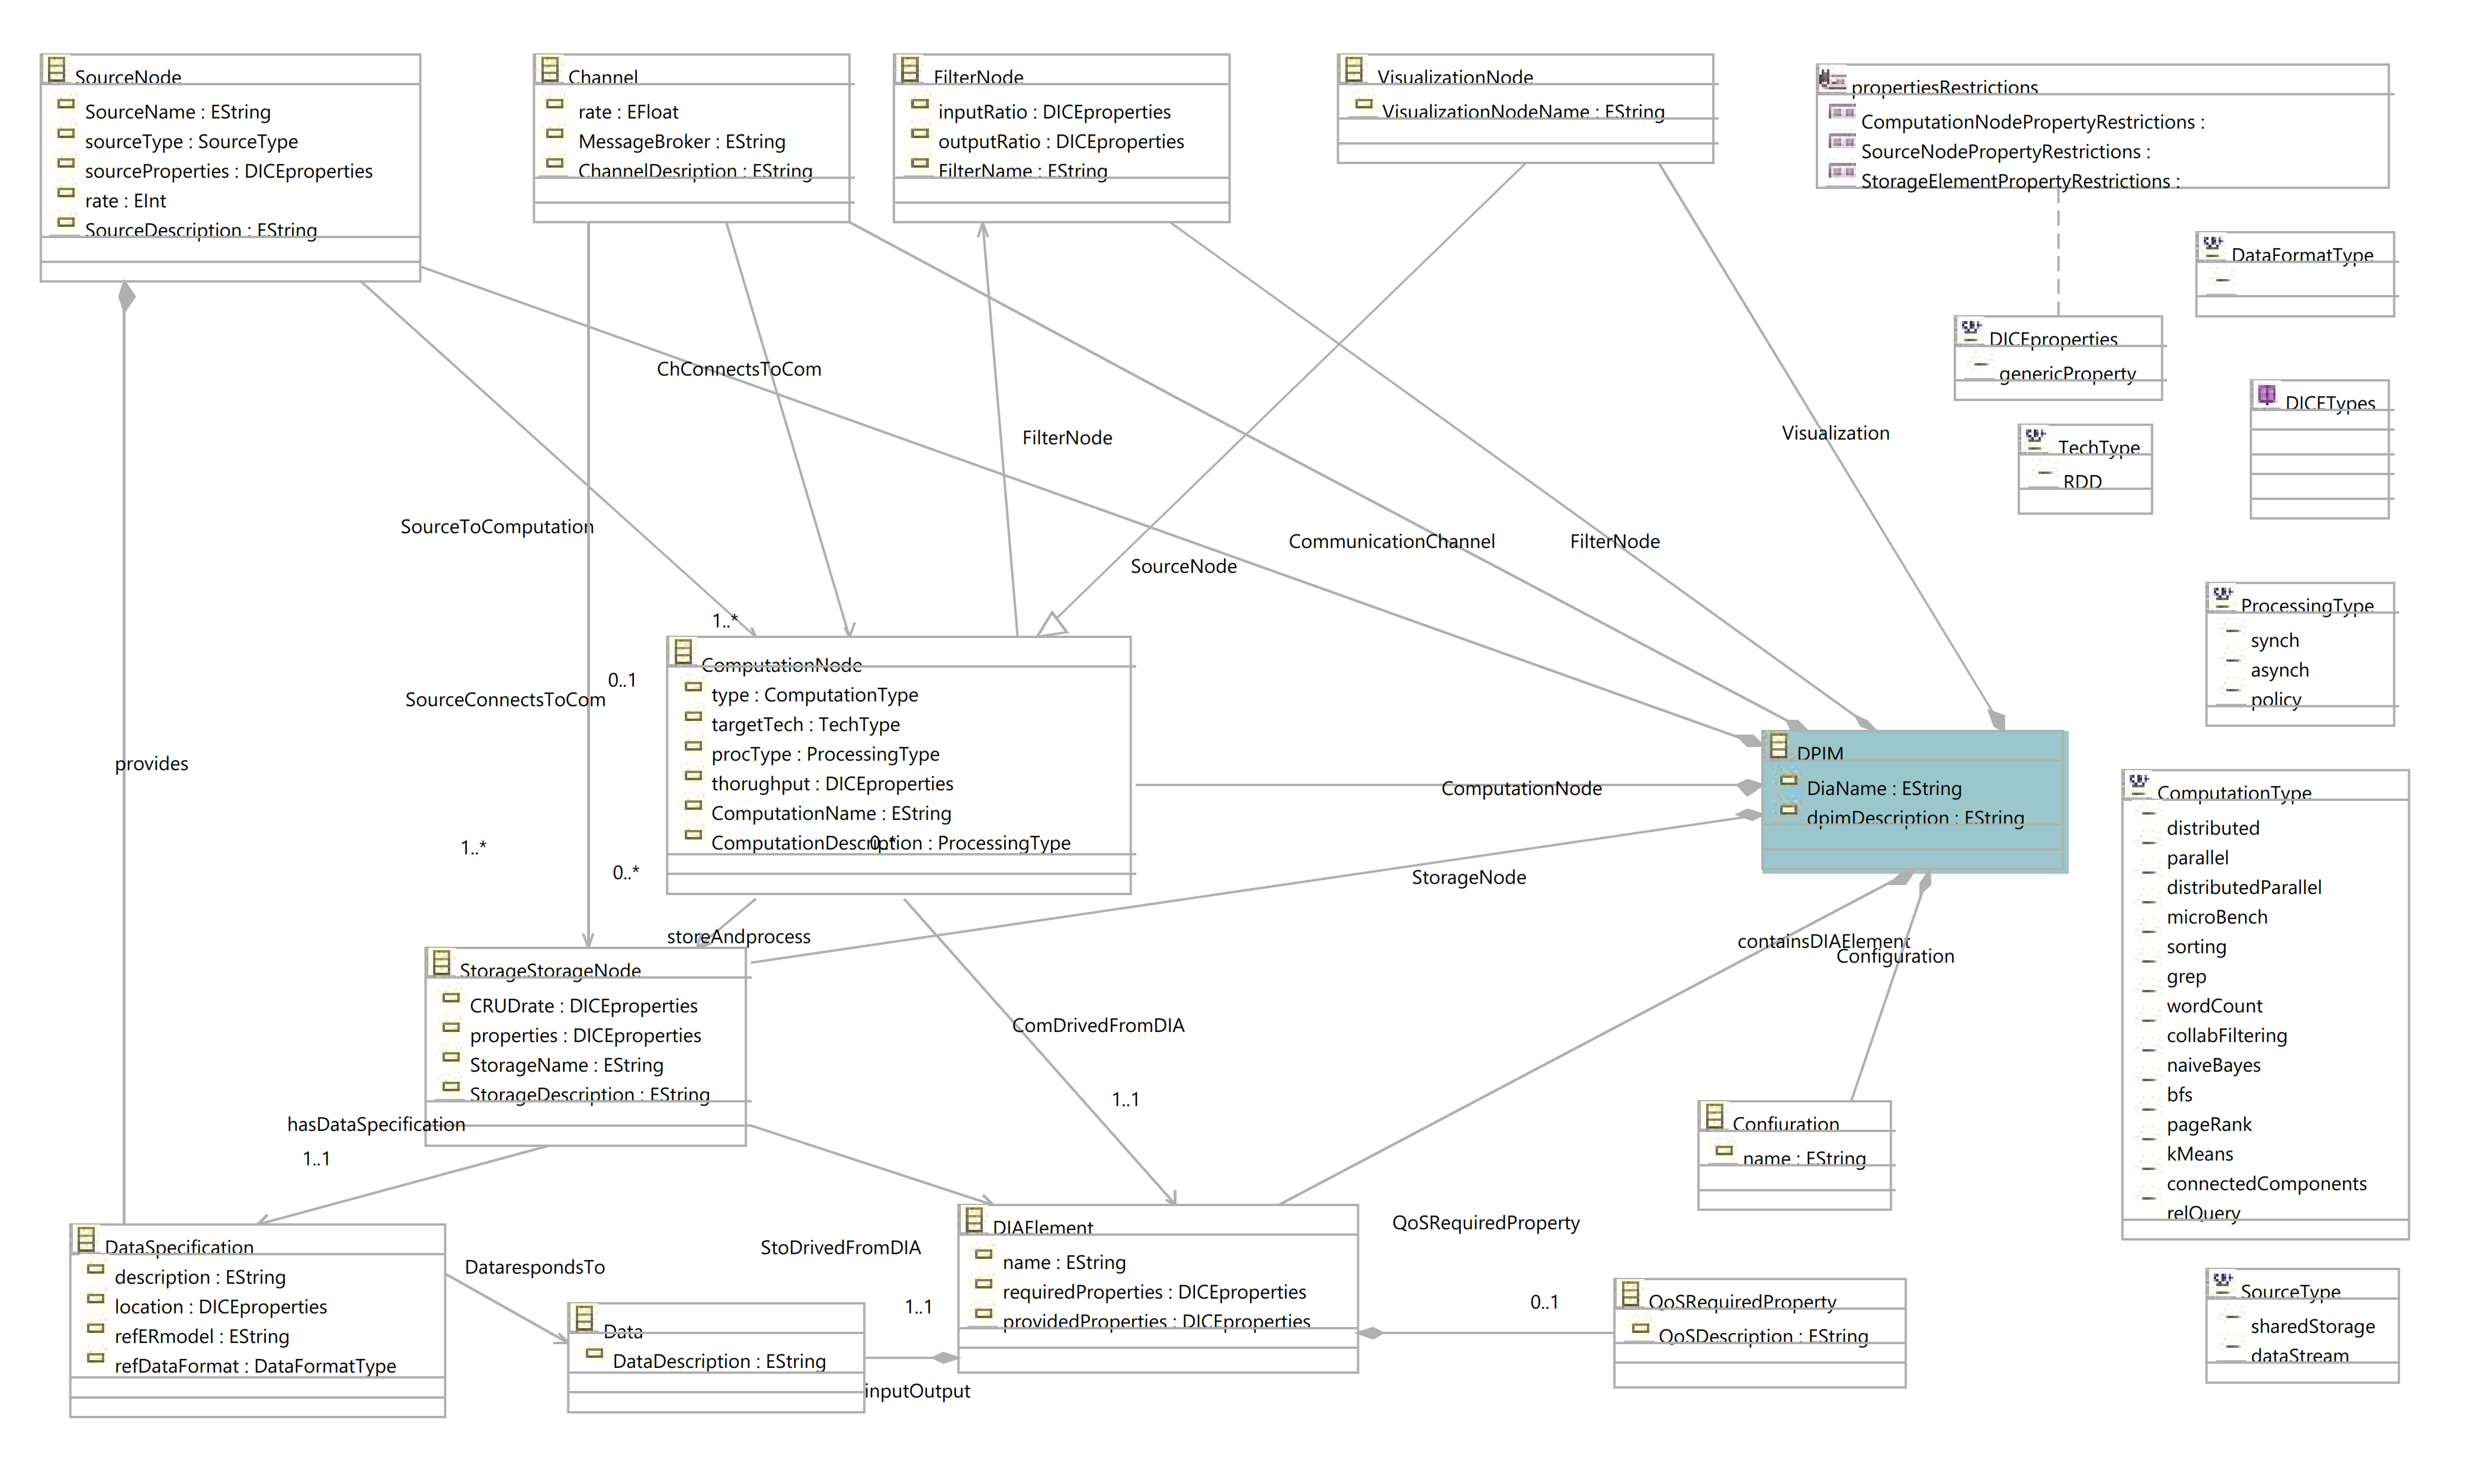
\includegraphics[width=\textwidth]{Images/11.png}
\caption{\label{fig:metamodel}DICE DPIM metamodel.}
\end{sidewaysfigure}

\begin{figure}
\centering
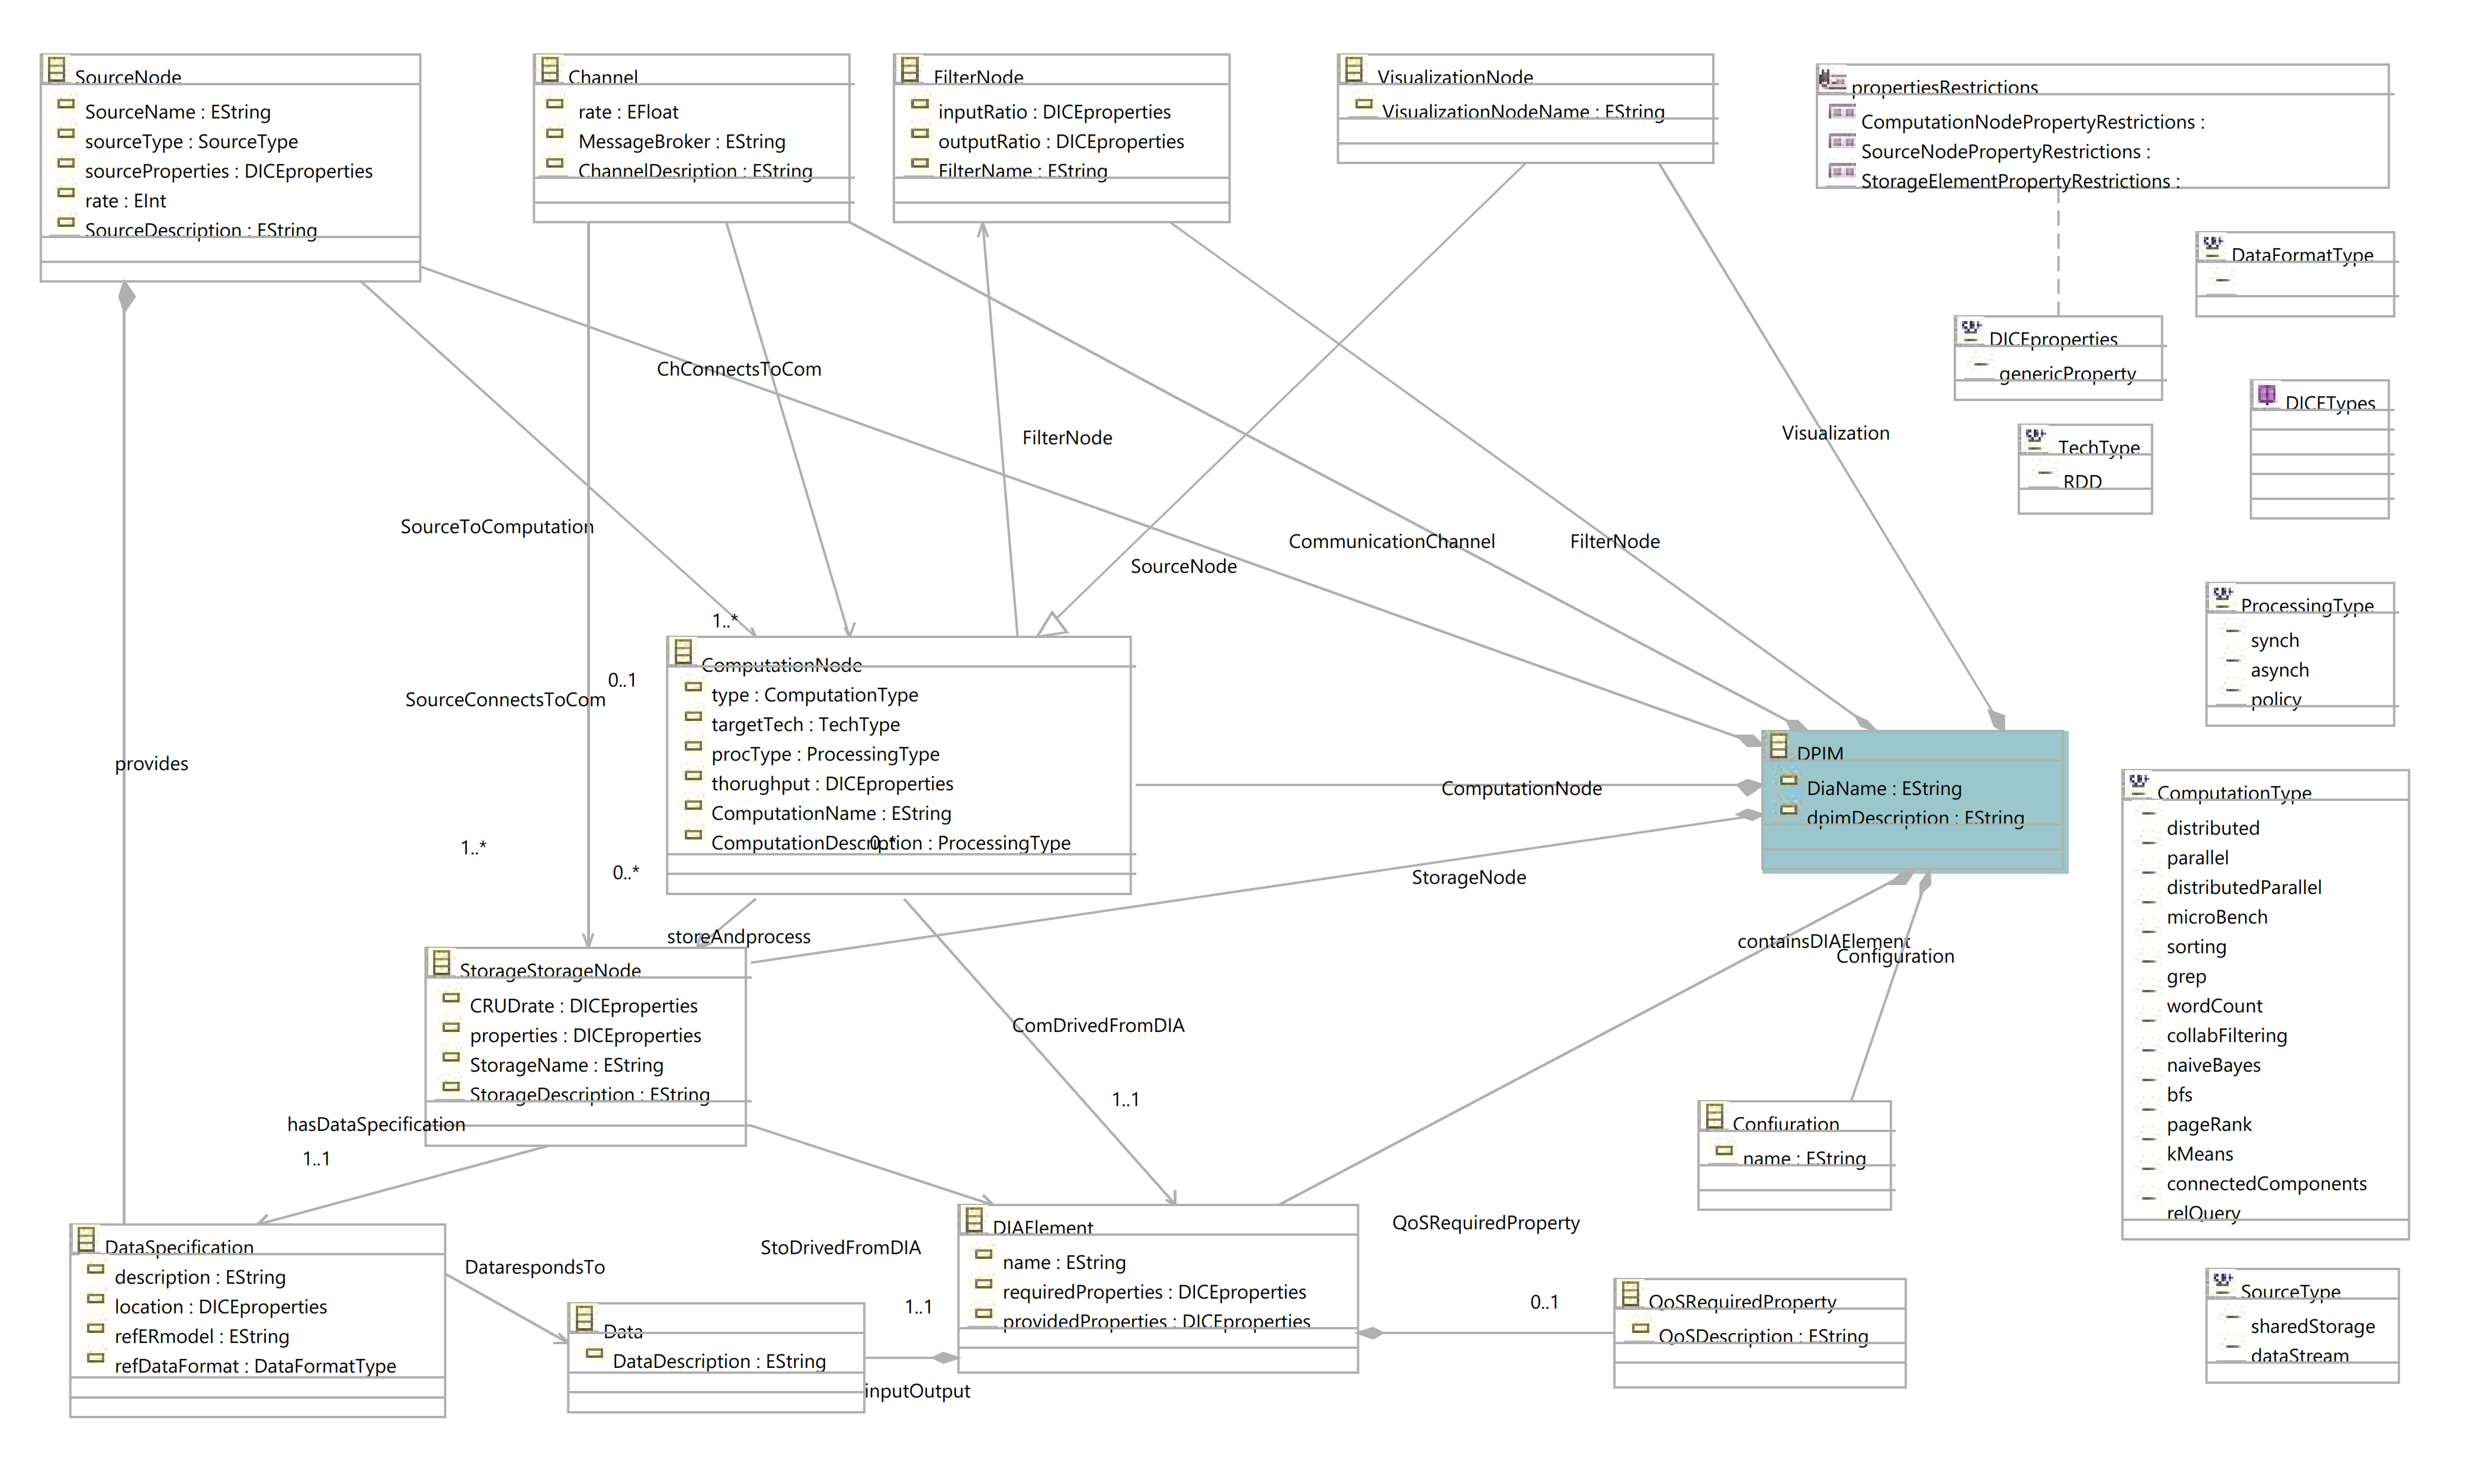
\includegraphics[width=\textwidth]{Images/11.png}
\caption{\label{fig:metamodel2}DICE DPIM metamodel in portrait form.}
\end{figure}
